\section{AI生成式绘画}\label{sec:painting}
在绘画领域,GPT不仅为创作者提供了强大的技术支持,还通过其生成能力,极大地拓展了绘画创作的边界。它能够实现多种复杂的图像操作,从生成创意草图到辅助完成细节绘制,为艺术家们提供了全新的创作思路和工具。这种技术与艺术的深度融合,不仅推动了绘画创作方式的变革,也为艺术表现形式带来了前所未有的可能性,进一步丰富了当代艺术的内涵与外延。

利用 GPT 的图像超分辨率技术,可以将低分辨率(1k)的图像无损地提升至高分辨率(4k)。这一过程通过深度学习算法对图像中的细节进行智能补充和重建,使得原本模糊的图像变得更加清晰锐利,满足对高清图像的需求,比如在印刷、大型展示等场景下的应用。GPT 可以精准识别图像主体与背景,通过算法自动去除背景,留下干净的主体图像。这对于需要将主体单独提取出来用于合成、设计等工作非常方便,大大节省了手动抠图的时间和精力。只需简单的指令,GPT 就能将图像的颜色进行反转,即黑变白、白变黑,其他颜色也相应反转。这种操作在一些创意设计、艺术创作中能带来独特的视觉效果,也有助于图像分析等工作。
当图像存在噪点影响视觉效果时,GPT 能够运用其去噪算法,智能识别并去除噪点,使图像恢复清晰、平滑,提升图像质量。用户可以向 GPT 输入想要替换的背景描述,如 “将当前图像背景替换为蓝天白云的草原场景”,GPT 会根据描述生成新的背景,并与原图像主体完美融合,创造出全新的画面效果。同样,若要替换图像中的人物,只需提供新人物的特征描述,如 “将画面中的人物换成一位穿着古装的女子”,GPT 就能完成人物替换,同时保证整体画面的协调性和逻辑性。无论是想要一张科幻风格的城市夜景图,还是温馨的家庭生活场景图,只要给出详细的需求,如 “生成一张未来城市中飞行汽车穿梭的图片,城市中有绚丽的霓虹灯和高楼大厦”,GPT 就能按照要求生成满足特定需求的高质量图片。GPT 可以根据文本描述生成各种想象中的场景。比如,当输入 “生成一个古代仙侠世界中的神秘山谷,山谷中有清澈的溪流、奇形怪状的石头和盛开的花朵”,它能迅速构建出相应的场景画面,为绘画创作者提供丰富的灵感和基础素材,大大加快创作进程。用户可以指定将一种图像风格迁移到另一种图像上。例如,将梵高的油画风格应用到一张普通的风景照片上,GPT 会分析梵高油画的笔触、色彩特点等,然后将这些风格元素融入到目标图像中,使其具有梵高油画的独特艺术风格。

\subsection{内容生成}

下面以liblib\footnote{\url{https://www.liblib.art}}为例演示AI生成图片的过程。首先在页面中选择合适的模型并输入提示词,该工具会自动将提示词转换为英文,最终得到生成的图片。

\prompt{设计一座未来主义风格的生态城市中心,融合高科技与可持续发展理念。建筑外观采用流线型结构,表面覆盖智能玻璃幕墙,能够根据天气和光线自动调节透明度。建筑内部设有垂直花园和空中花园,以最大化绿化空间。屋顶配备太阳能板和雨水收集系统,以实现能源自给自足和水资源循环利用。整体风格简洁而富有科技感,同时融入自然元素,营造出人与自然和谐共生的未来城市景观。}

\begin{gptbox}
s \footnotesize{以下是生成的图片:}
\fig[H]{
    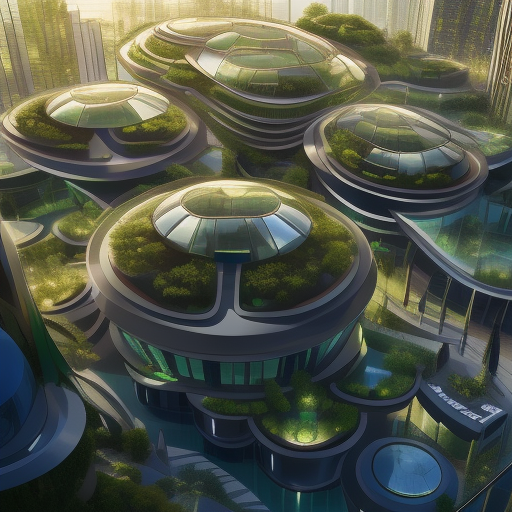
\includegraphics[width=0.3\textwidth]{gc}
}
\end{gptbox}


\subsection{图像风格转移}

在探索人工智能辅助图像编辑的前沿领域时,一个值得关注的工具是InstructPix2Pix。该模型由Hugging Face\footnote{\url{https://huggingface.co}}平台上的开发者timbrooks创建,能够根据用户输入的提示词对图像进行修改和变换,从而实现高度定制化的图像生成。用户可以通过访问InstructPix2Pix - a Hugging Face Space by timbrooks进入该模型的交互界面,如\reffig{fig:gc-InstructPix2Pix}所示。

在使用该工具时,用户首先需要上传待修改的图像,这一操作以红色框标出。随后,用户需在蓝色框中输入提示词,以描述期望的图像修改效果。为确保最佳效果,建议使用英语,并尽可能以简洁明了的方式表达需求。此外,界面中的绿色框提供了参数调整选项,其中“Text CFG”和“Image CFG”是两个关键参数。Text CFG用于调节提示词的权重,而Image CFG则用于调整图像本身的权重。用户可以通过对这两个参数的精细调整来实现预期的图像效果。然而,需要注意的是,这两个参数之间必须保持适当的平衡。如果Text CFG权重过高,可能导致生成的图像与原始图像失真;而如果Image CFG权重过高,则可能使生成的图像无法完全符合提示词的要求。因此,用户在使用过程中需要根据具体需求灵活调整参数,以达到理想的效果。

\fig[h]{
    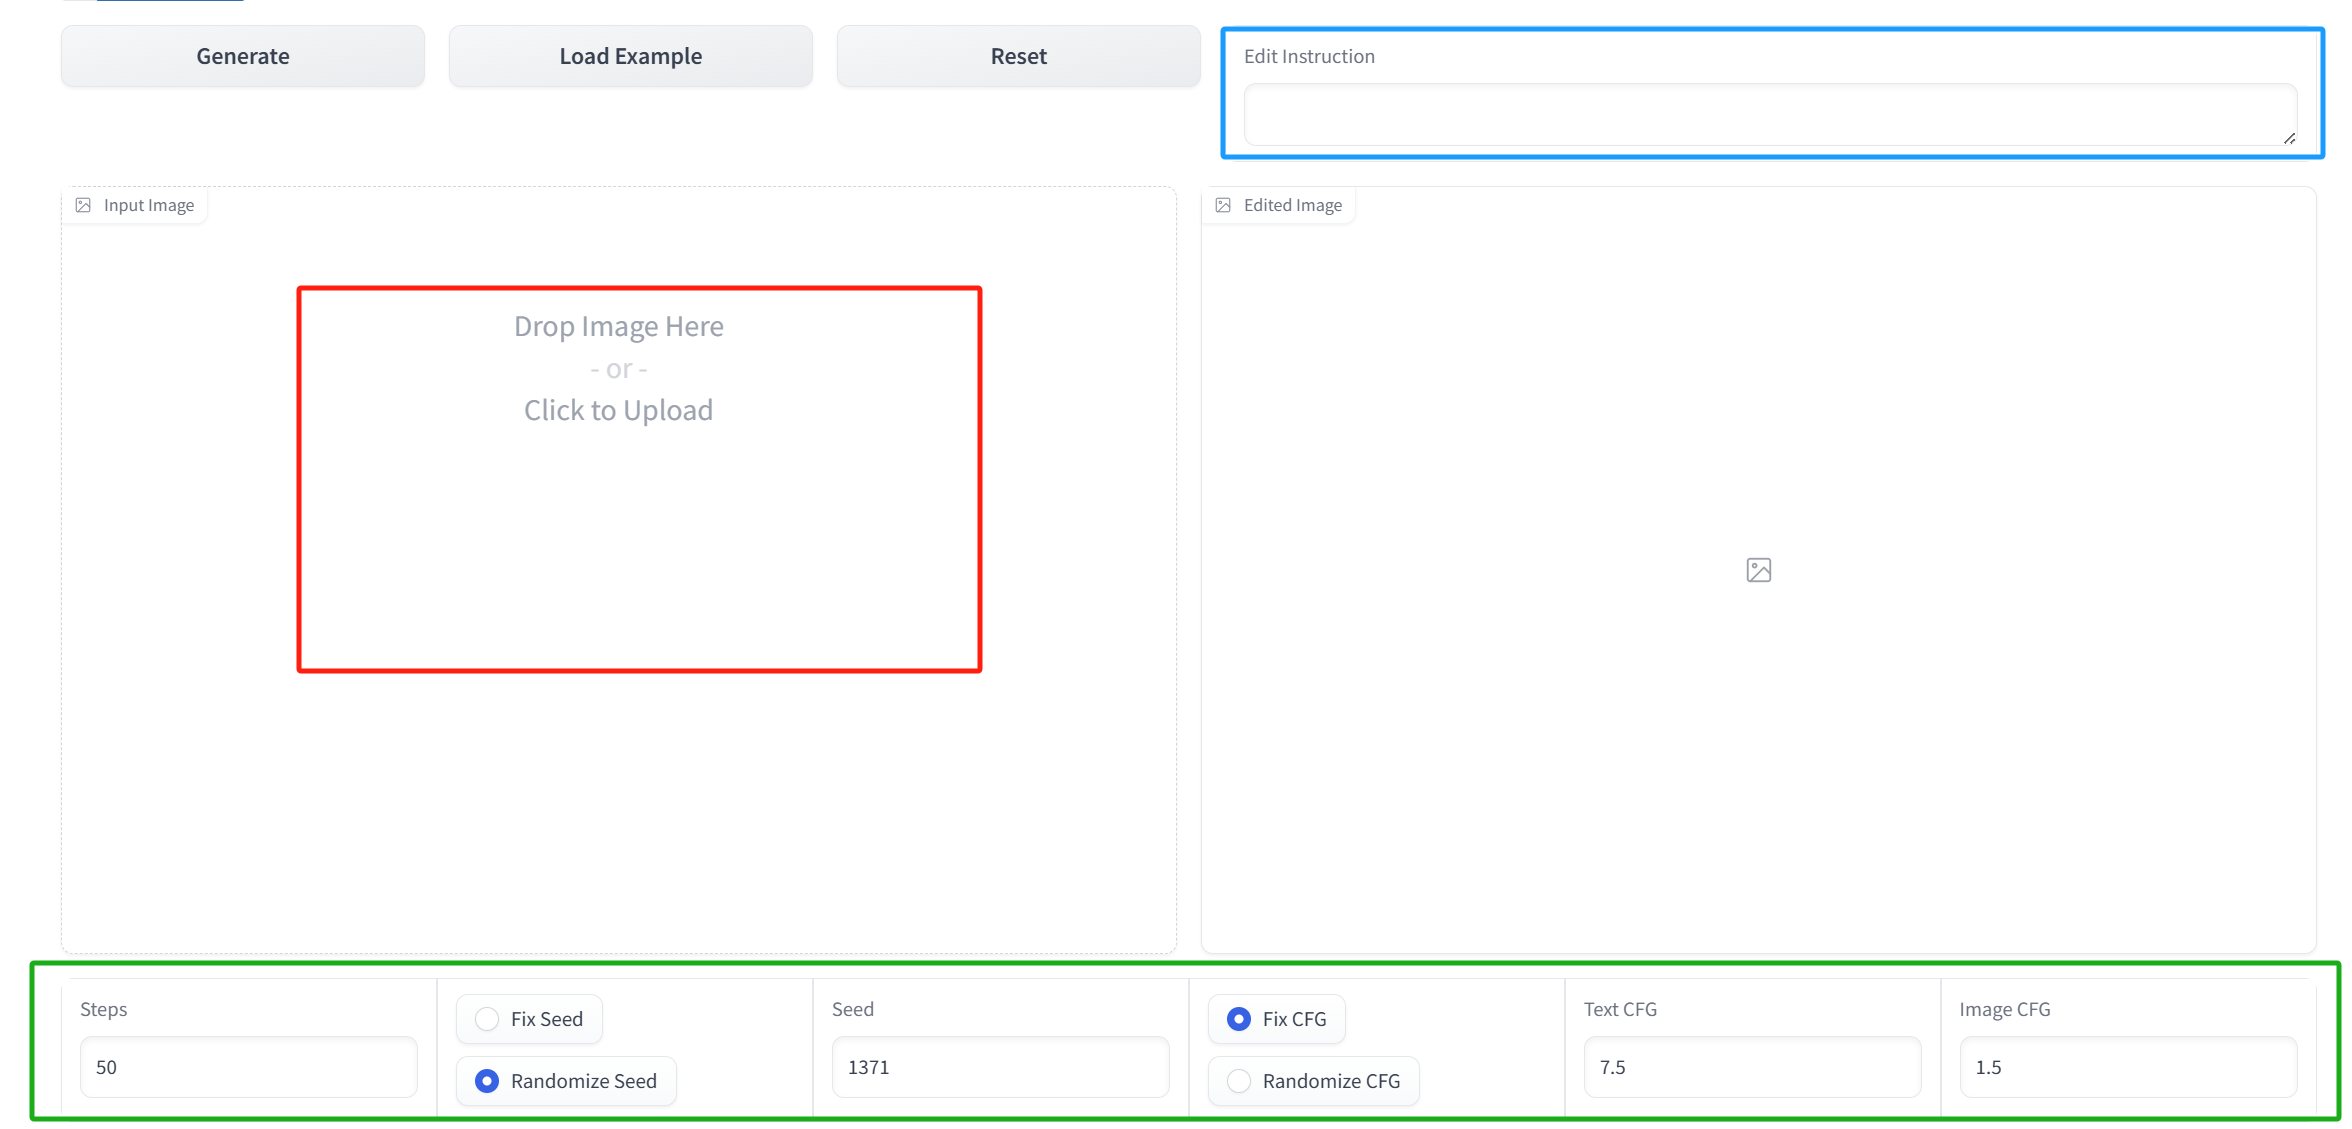
\includegraphics[width=0.7\textwidth]{assets/figures/image-20250211145347208.png} %插入图片,[]中设置图片大小,{}中是图片文件名
    \caption{InstructPix2Pix参数调整} %最终文档中希望显示的图片标题
    \label{fig:gc-InstructPix2Pix} 
}

例如,若需将云南师范大学的校园照片转化为动漫风格,可通过精心设置相关参数并输入恰当的提示词来实现这一风格转换,如\reffig{fig:gc-rendering}和\reffig{fig:gc-rendered}所示。

\fig[h]{
    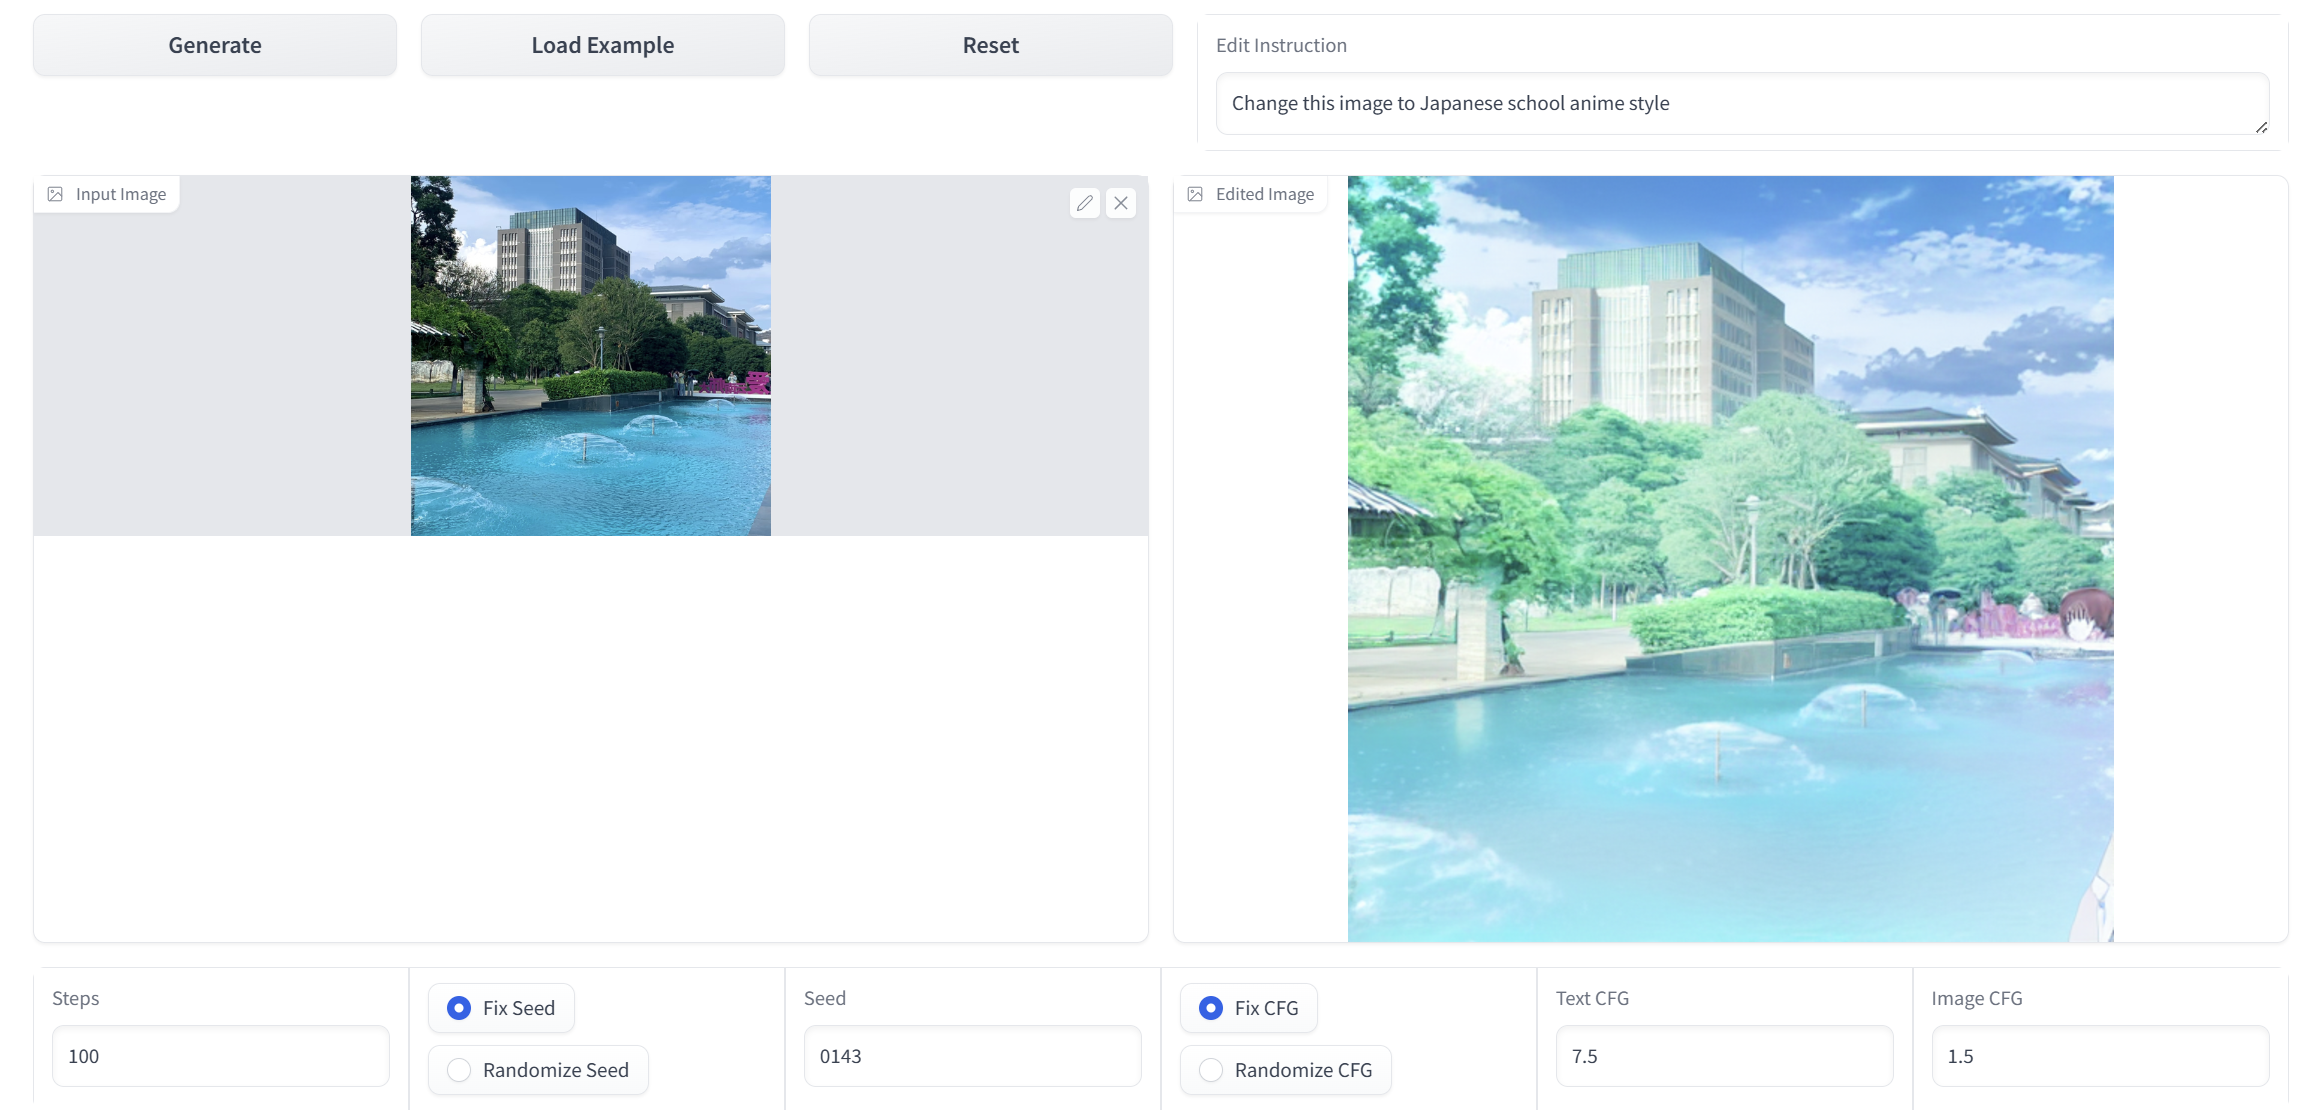
\includegraphics[width=0.7\textwidth]{assets/figures/9c6c2ff0409374eed093b8ec3447507.png} %插入图片,[]中设置图片大小,{}中是图片文件名
    \caption{渲染过程} %最终文档中希望显示的图片标题
    \label{fig:gc-rendering} 
}

\fig[h]{
    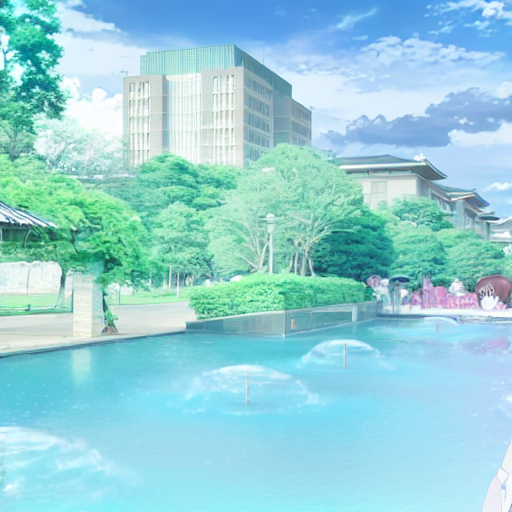
\includegraphics[width=0.7\textwidth]{assets/figures/change.png} %插入图片,[]中设置图片大小,{}中是图片文件名
    \caption{渲染效果图} %最终文档中希望显示的图片标题
    \label{fig:gc-rendered} 
}

通过对比两幅图像,可以清晰地观察到其风格上的显著差异。在此基础上,用户可进一步调整参数,以不断优化并最终实现预期的图像效果。



